\section{Basic probability theory}
\thispagestyle{plain}

Scientists measure things, for instance the (adult) length of a species of fish.
Very natural questions might be
\begin{itemize}
    \item How probable are certain (ranges) of lengths? - so how is the fish-length \textit{distributed}
    \item What is the average length? And given we have measured $8$ fish, how sure can we be that our average
    is a good proxy to the whole population average? So if I measured $8$ other random fishes, how much would their
    average length differ? Things probably get better the more fish we measure \dots
    \item How is the fish length related to other measurements we did? For instance the enrichment of nutrients in the water?
\end{itemize}

Let us start with basic definitions and distributions.

\subsection{Basic definitions}
A probability model is given by $\{\Omega,E,P\}$ with
\begin{itemize}
    \item sample space $\Omega$, e.g. all possible fish lengths
    \item events $E$, e.g. a length measured $> 5\cm$
    \item probability $P$ of an event
\end{itemize}

\subsubsection{Sample space $\Omega$}
This is the set of fundamental outcomes in our experiment
\begin{itemize}
    \item for rolling $1$ dice: $\{1,\dots,6\}$
    \item for rolling $2$ dice: $\{(1,1),(1,2),\dots,(6,6)\}$
\end{itemize}

\subsubsection{Set of events $E$ defined on the sample space}
Examples for events could be
\begin{itemize}
    \item for rolling $1$ dice: $A_1:=\{2,4,6\}$ (even result), $A_2 := \{1,3,5\}$ (odd result)
    \item for our fish lengths: $A:=\{l:l\geq 6 \cm\}$.
\end{itemize}
more precisely, \textcolor{blue1}{$E$ needs to be a $\sigma$-algebra} that
\begin{itemize}
    \item $E$ contains the sample space $\Omega$
    \item $E$ is closed under complementation: $A \in E \rightarrow \bar{A} \in E$
    \item $E$ is closed under countable untions: if $\{A_i\}_{i=1}^K \in E$ then $\cup_{i=1}^K A_i \in E$
\end{itemize}
The smallest set of events is $\{\emptyset,\Omega\}$, the smallest one containing a subset
$A \subseteq \Omega$ is $\{\emptyset,\Omega, A, \bar{A}\}$.

\subsubsection{Probability measure $P$}
A probability measure maps events to a probability, so $P:E\rightarrow [0,1]$ with
\begin{itemize}
    \item $P(A) \geq 0 \, \forall A \, \in E$
    \item $P(\Omega) = 1$
    \item for any $A_i,A_j \in E$ such that $A_i \cap A_j = \emptyset$ (are disjoint)
    \begin{equation}
        P\left(\bigcup_{i=1}^K A_i\right)=\sum_{i=1}^K P\left(A_i\right)
    \end{equation}
    (probabilities of disjoint sets just add)
\end{itemize}
\subsubsubsection{Examples for the probabilities of events | discrete and continuous situations}
\begin{itemize}
    \item for $1$ dice: $A_1 = \{2,4,6\}, A_2 = \{ 1, 3, 5 \} \rightarrow P(A_1) = P(A_2) = \frac{1}{2}$
    \item for $2$ dice (where order matters): $\Omega = \{(c_1,c_2)|c_1,c_2 \in \{1,\dots,6\}\}, |\Omega| = 36$, e.g.
    \begin{itemize}
        \item $A = \{c_1 = c_2\} \rightarrow P(A) = \frac{6}{36} = \frac{1}{6}$
        \item $B = \{c_1+c_2 \geq 10\} = \{(5,6),(6,5),(6,6) \} \rightarrow P(B) = \frac{1}{12}$
    \end{itemize}
    \item continuous situation: $x \in \mathbb{R}$, e.g.
    \begin{itemize}
        \item $A={x\leq b}, P(A) = P(x\leq b) = \int_{-\infty}^{b} f(x) \, dx$ where $f$ is the probability density function (PDF)
    \end{itemize}
\end{itemize}

\subsection{Basic probability laws}
Let $A,B \in E$ with $E$ a $\sigma$-algebra.
\subsubsection{Conditional and joint probability}
The probability of $A$ when $B$ has already occurred is called
conditional probability $P_B(A) = P(A|B)$.

Naturally the intersection of two sets of events $A \cap B$
has the \textit{joint probability} (\enquote{path-rule})

\begin{equation}
    \label{eq:joint_probability}
    \boxed{P(A,B) := P(A \cap B) = P(B) P(A|B) = P(A) P(B|A) \quad \rightarrow \quad P(A|B) = \frac{P(A,B)}{P(B)}}
\end{equation}

so the general joint probability is

\begin{equation}
    P(A_1,A_2,\dots,A_K) = P(A_1) P(A_2 | A_1) P(A_3|A_1,A_2) \cdot \dots \cdot P(A_K|A_1,\dots,A_{K-1})
\end{equation}

The path rule is illustrated in figure \ref{fig:path_rule}.

\begin{figure}[!htb]
    \centering
    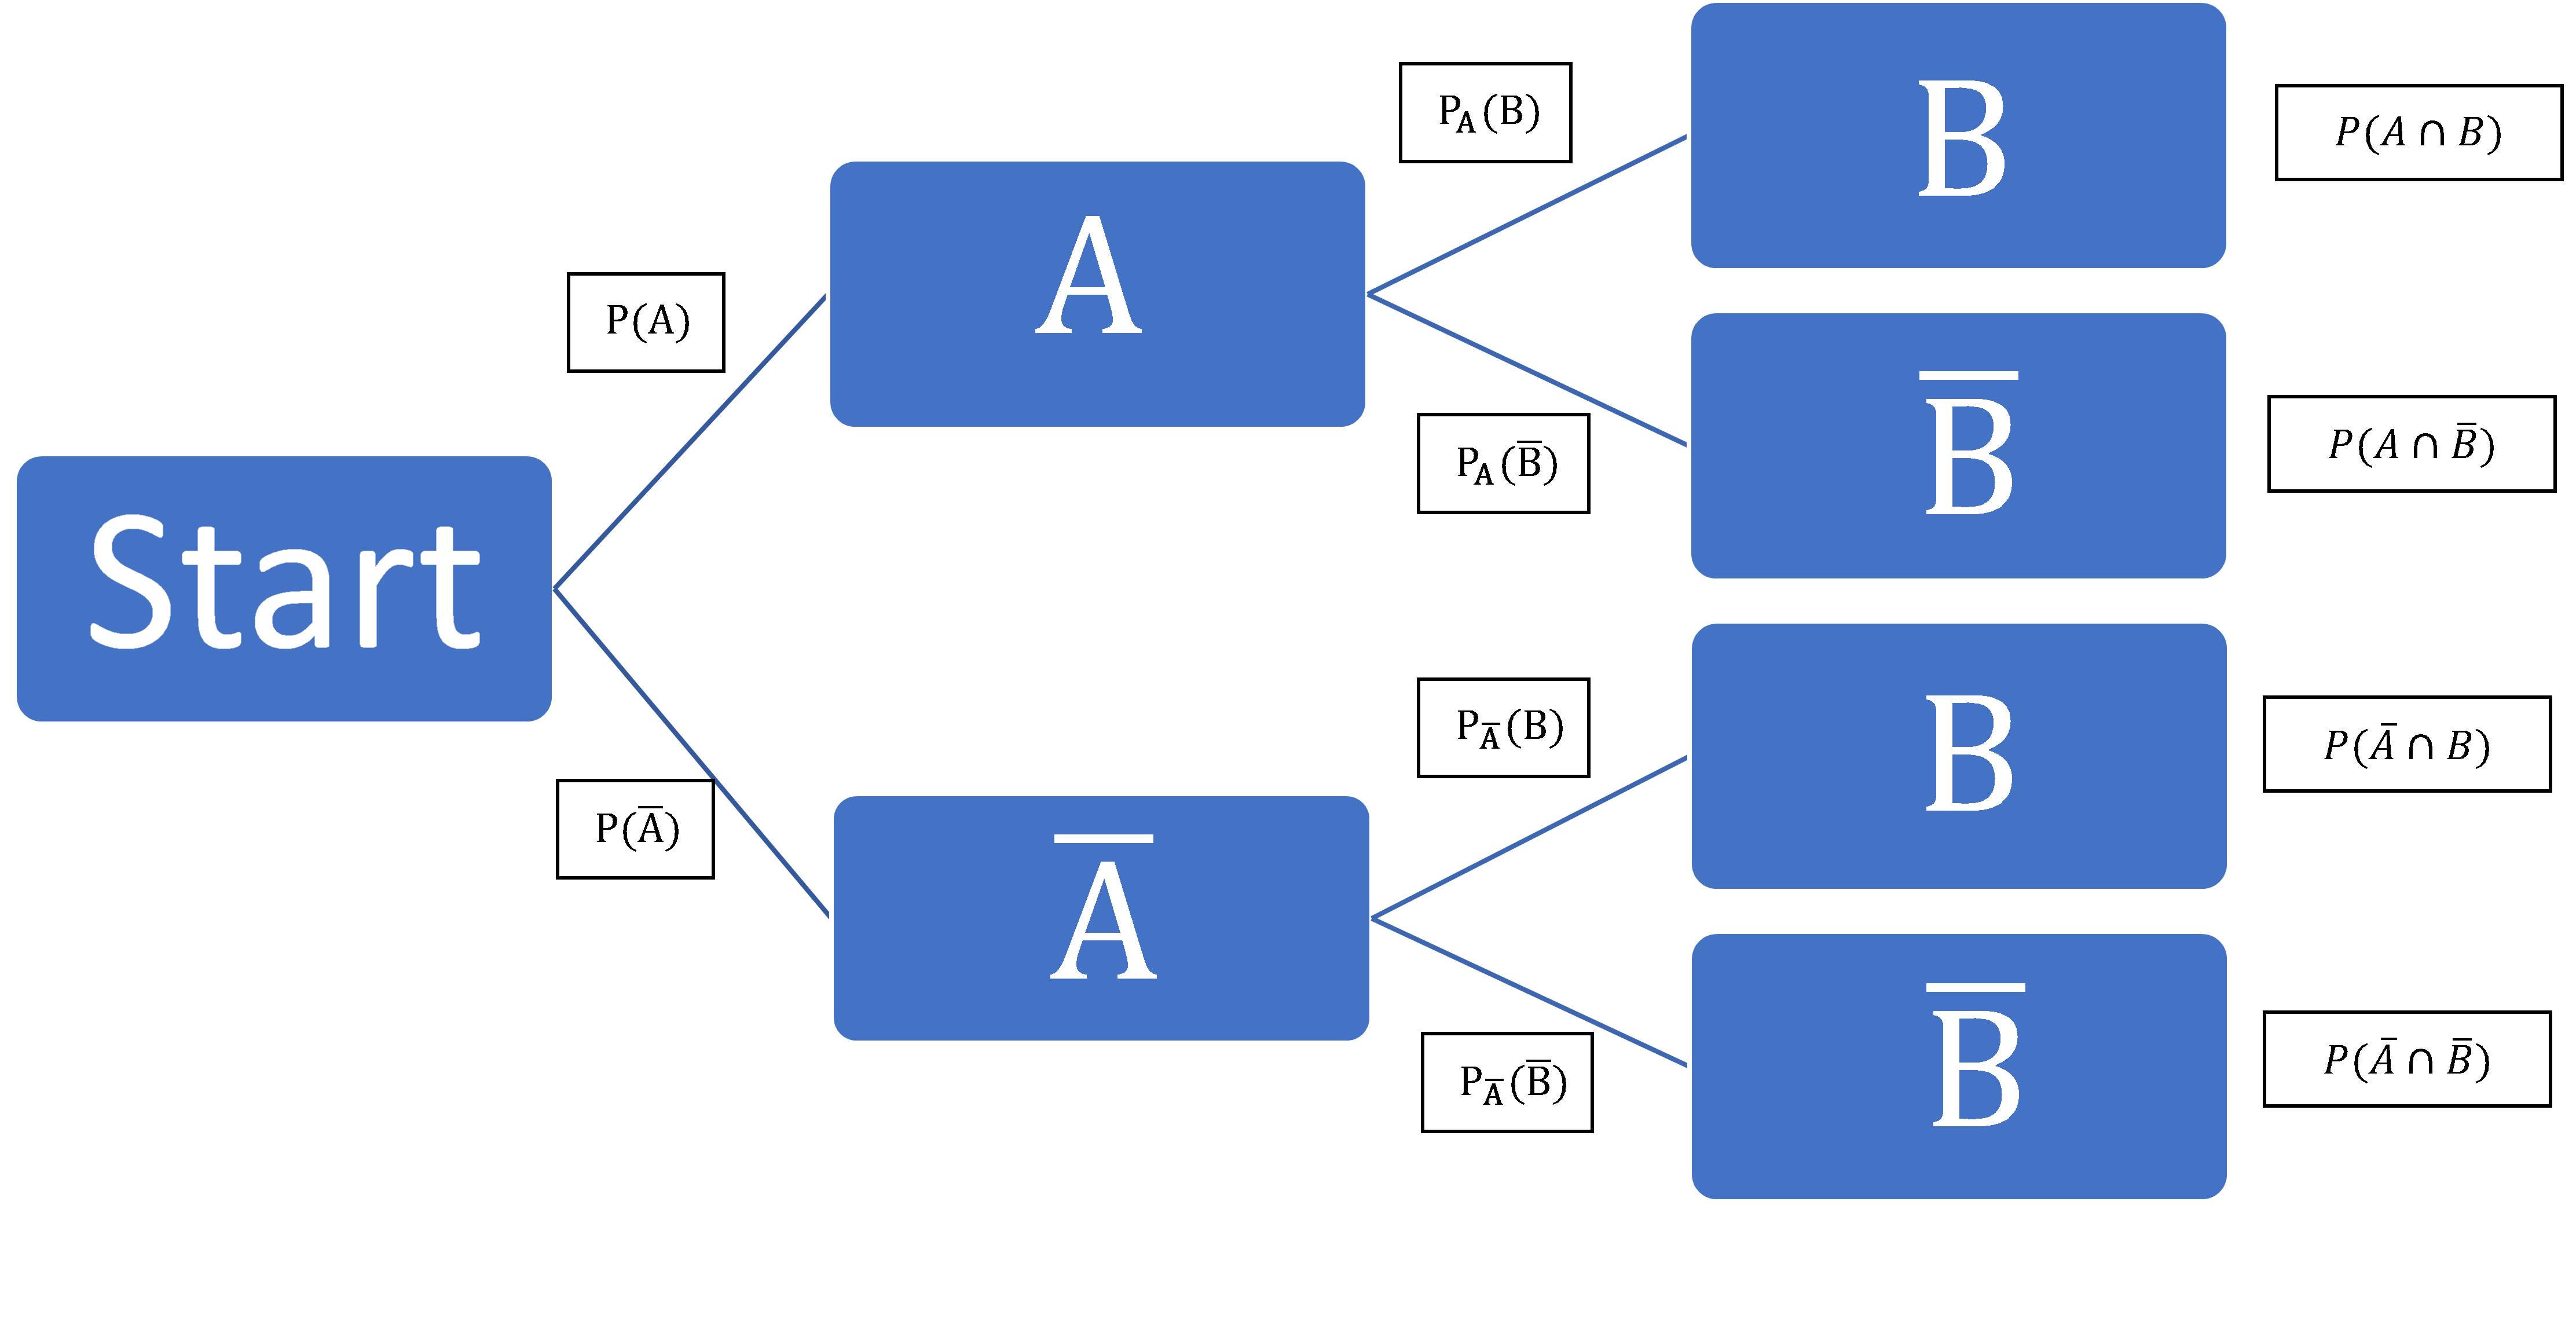
\includegraphics[width=0.9\textwidth]{figures/path_rule.png}
    \caption{Path rule for joint probability}
    \label{fig:path_rule}
\end{figure}

\subsubsection{Bayes rule}
From eq. \ref{eq:joint_probability} we can follow Bayes rule
\begin{equation}
    P(H \mid E)=\frac{P(E \mid H) \cdot P(H)}{P(E)}, \quad P(E \mid H)=\frac{P(H \mid E) \cdot P(E)}{P(H)}
\end{equation}
with
\begin{itemize}
    \item \textbf{hypothesis $H$}: a hypothesis which probability may be affected by evidence $E$
    \item \textbf{prior probability $P(H)$}: the probability of the hypothesis before the evidence is observed
    \item \textbf{likelihood $P(E \mid H)$}: the probability of the evidence given that the hypothesis is true
    \item \textbf{probability of evidence $P(E)$}: (aka marginal likelihood) the probability of obtaining the evidence generally. When we are likely to obtain the evidence independent of the hypothesis, it does not confidently support any hypothesis
    \item \textbf{posterior probability $P(H \mid E)$}: the probability of the hypothesis after the evidence is observed
\end{itemize}

\subsubsection{Probability of the union of events}
Additive laws are shown in table \ref{tab:additive_laws}.

% create a latex table with top field venn digram (one figure)
% and below two fields with the additive laws
\begin{table}[!htb]
    \centering
    \begin{tabular}{|p{0.95\textwidth}|}
        \hline
        Venn diagram \\
        \includesvg[width=0.95\textwidth]{figures/venn.svg} \\
        \hline
        \begin{tabular}{p{0.45\textwidth}|p{0.45\textwidth}}
            \begin{equation}
                P(A \cup B) = P(A) + P(B) - P(A,B)
            \end{equation} &
            \begin{equation}
                \begin{gathered}
                    P(A \cup B \cup C) \\= P(A) + P(B) + P(C) \\
                    - P(A,B) - P(A,C) - P(B,C) \\ + P(A,B,C)
                \end{gathered}
            \end{equation}
        \end{tabular} \\
        \hline
    \end{tabular}
    \caption{Additive laws}
    \label{tab:additive_laws}
\end{table}

\subsubsection{Independent events}
Two events $A$ and $B$ are independent if and only if
\begin{equation}
    P(A,B) = P(A) P(B)
\end{equation}
so their joint probability is the product of the marginals,
which follows if
\begin{equation}
    P(A|B) = P(A) \quad \text{or} \quad P(B|A) = P(B)
\end{equation}
so for the occurrence of event $A$ it does not matter if $B$ has already occurred
and vice versa.
\subsubsection{Example for throwing one dice (once)}
For a dice $\Omega = \{1,\dots,6\}$. Consider events $A = \{1,3,5\}$ and $B = \{2,4,6\}$ and $C = \{1,2\}$.

\begin{itemize}
    \item We can readily see that $A$ excludes $B$ and vice versa (fully dependent), $P(A) = P(B) \frac{1}{2}$ and
    $P(A|B) = 0$ so $P(A,B) = P(B) P(A|B) \neq P(A) \cdot P(B)$.
    \item $A$ and $C$ as well as $B$ and $C$ are independent - having obtained a $1$ or $2$ the probability that
    it is a $1,3$ or $5$ is $\frac{1}{2}$ just as for obtaining a $1$, $3$ or $5$ in the first place.
\end{itemize}

\subsubsection{Probability of the complement}
\begin{equation}
    P(\bar{A}) = 1 - P(A)
\end{equation}

\greenbox{\textbf{The complement can be very useful}:
Consider from integers up to $N$ you draw $N$ numbers (repititions allowed), so
\begin{equation}
    \Omega_0 := \{1,2,\dots,N\}, \quad P(\omega_i \in \Omega_0) = \frac{1}{N}
\end{equation}
\textbf{Question:} What is the probability $P(A)$ that at least two numbers are the same? - 
The probability that all numbers are different is the fraction of possible different draws
$N!$ divided by all possible arrangements $N^N$, so $P(A) = 1 - \frac{N!}{N^N}$.
}

\subsubsection{Law of total probability | marginalization}
Given the joint $P(A_i \cap B) = P(A_i,B); A_i,B \subseteq \Omega$ how can we obtain $P(B)$?

If the $A_i$ are a pairwise disjoint partition of $\Omega$ so

\begin{equation}
    \bigcup_{i=1}^K A_i=\Omega, \quad \forall i \neq j: A_i \cap A_j=\varnothing
\end{equation}

then we can marginalize out the $A_i$ by

\begin{equation}
    P(B)=\sum_{i=1}^K P\left(A_i\right) \cdot P\left(B \mid A_i\right)=\sum_{i=1}^K P\left(A_i, B\right)
\end{equation}

\note{Therefore, we can write the probability of the evidence in Bayes law as
\begin{equation}
    P(E) = \sum_{i=1}^K P\left(H_i, E\right) = \sum_{i=1}^K P(H_i) \cdot P\left(E \mid H_i\right)
\end{equation}
-\textit{marginalized likelihood}.
}

\subsection{Random Variables (RVs)}
Strictly, a random variable $X$ is neither random nor a variable.
\bluebox{A random variable $X$ is a mapping or function $X:\Omega \rightarrow F$ from possible outcomes
(from a sample space, e.g. $\Omega = \{\text{Head},\text{Tail}\}$ for a coin) to
a measurable space $F$ (e.g. $\{-1,1\}$, $1$ for heads, $-1$ for tails).}

\subsubsection{Examples for random variables}
\begin{itemize}
    \item for two dice with $\Omega = \{(c_1,c_2)|c_1,c_2 \in \{1,\dots,6\}\}$, e.g. $X = c_1 + c_2$ is a random variable
    \item the length of a randomly measured fish
    \item for $8$ randomly measured fishes, the mean length is also a random variable - \textbf{estimators themselves are
    random variables} and hence have a distribution, a mean, a variance, and so on with a particular realization of this random number
    called \textit{estimate}
    \item \dots
\end{itemize}

\subsubsection{Continuous and discrete Random variables}
A random variable $X$ comes with its probability distribution.

Discrete random variables have a probability mass function (PMF)
$P(X = X_i) = p(x_i)$ while continuous random 
variables have a probability density function
$f(x)$ where formally any specific $x$ has probability
zero but ranges have probabilities, cumulative density (CDF) $P(X<x_0) = \int_{-\infty}^{x_0}
f(x) \, dx$. PMF and PDF are normed.

\subsubsection{Expectation values}
The expectation value is the first moment of the probability mass or density
function.

\begin{equation}
    \begin{gathered}
    E[X] \underset{X \text { discrete }}{=} \sum_{i=1}^N P\left(X=x_i\right) x_i \\
    \underset{X \text { continuous }}{=} \int_D f(x) x d x
    \end{gathered}
\end{equation}

\subsubsubsection{Properties of the expectation value}
\begin{itemize}
    \item expectation value of $c = \text{const.} \rightarrow E[c] = c$
    \item linerity of the expectation value: Let $\{x_i\}$ be a set
    of RVs and $\{c_i\}$ of constants, then
    \begin{equation}
        E\left[\sum c_i x_i\right]=\sum c_i E\left[x_i\right]
    \end{equation}
    \textcolor{blue1}{Proof}: For two variables, this follows from
    \begin{equation}
        \begin{aligned}
        E\left[c_1 x_1+c_2 x_2\right]&=\sum_{x_1} \sum_{x_2}\left(c_1 x_1+c_2 x_2\right) P\left(x_1, x_2\right) \\
                                     &=c_1 \sum_{x_1} x_1 \sum_{x_2} P\left(x_1, x_2\right)+c_2 \sum_{x_2} x_2 \sum_{x_1} P\left(x_1, x_2\right) \\
                                    \underset{\text { marginalization }}&= c_1 E\left[x_1\right]+c_2 E\left[x_2\right]
        \end{aligned}
    \end{equation}
    \item Expectation over a function $g(x)$
    \begin{equation}
        E\left[g\left(x_1, \ldots, x_N\right)\right]=\sum_{x_1} \ldots \sum_{x_N} p\left(x_1, \ldots, x_N\right) g\left(x_1, \ldots, g_N\right)
    \end{equation}
    \item multiplicativity in case of independence: for $X,Y$ independent
    \begin{equation}
        p\left(x_1, x_2\right)=p\left(x_1\right) p\left(x_2\right) \rightarrow E\left[g_1\left(x_1\right) g_2\left(x_2\right)\right]=E\left[g_1\left(x_1\right)\right] E\left[g_2\left(x_2\right)\right]
    \end{equation}
\end{itemize}

\subsubsubsection{Conditional expectation}
What is the expected value of a random variable $X$ if $Y = y$ has already occured?
\begin{equation}
    E[X \mid Y=y]=\sum_x x P(X=x \mid Y=y)=\sum_x x \frac{P(X=x, Y=y)}{P(Y=y)}
\end{equation}
so in the continuous case
\begin{equation}
    E[X|Y = y] = \int_{-\infty}^{\infty} f(x|y) \, x \, dx
\end{equation}
\note{Subscripts in expectation values are used ambiguously, $E_X[h(X,Y)]$
can mean the conditional expectation
\begin{equation}
    E_X[h(X, Y=y)]=E[h(X, Y=y) \mid X]=\sum_y h(x, y) p(h(x, y) \mid x)
\end{equation}
or a marginal density used for averaging
\begin{equation}
    E_X[h(X, Y=y)]=\sum_x h(x, y) p_X(x)
\end{equation}
}
\subsubsubsection{Law of total expectation}
Let us over the conditional expectation
\begin{equation}
    \mathcolor{blue1}{E_{X \mid Y}[X \mid Y] \text { is a random variable depending on } Y}
\end{equation}
take the expectation over $Y$
\begin{equation}
    E_Y\left[\mathcolor{blue1}{E_{X \mid Y}[X \mid Y]}\right]=E[X]
\end{equation}
following from
\begin{equation}
    \begin{aligned}
    E_Y\left[\mathcolor{blue1}{E_{X \mid Y}[X \mid Y]}\right]&=\mathcolor{green1}{E_Y\left[\mathcolor{blue1}{\sum_x x P[X=x \mid Y]}\right]}\\
    &=\mathcolor{green1}{\sum_y\left[\mathcolor{blue1}{\sum_x x P[X=x \mid Y=y]}\right] \cdot P(Y=y)} \\
    \underset{P(A \mid B)=\frac{P(A, B)}{P(B)}}&= \sum_y\left[\sum_x x P[X=x, Y=y]\right]\\
    &=\sum_x x \mathcolor{yellow1}{\sum_y P[X=x, Y=y]} \\
    \underset{y \text { is marginalized out }}&= \sum_x x \mathcolor{yellow1}{P[X=x]}=E[X] \\
    \end{aligned}
\end{equation}

\subsubsection{Variance, Covariance and Correlations}
\subsubsubsection{Variance}
The variance is the expected squared deviation from the mean, so
\begin{equation}
    \sigma^2=\operatorname{Var}(X)=E\left[(X-\mu)^2\right]=\sum_{i=0}^{\infty} p\left(X=x_i\right)\left(x_i-\mu\right)^2=\operatorname{Cov}(X, X), \quad \mu=E[X]
\end{equation}
\bluebox{For calculating the variance the following relations
\begin{equation}
    \operatorname{Var}(X)=E\left[(X-E[X])^2\right]=E\left[X^2-2 X E[X]+E[X]^2\right] \underset{E \text { linear }}{=} E\left[X^2\right]-E[X]^2
\end{equation}
and
\begin{equation}
    a, b=\text { const }: \quad \operatorname{Var}[a x+b]=a^2 \operatorname{Var}[x]
\end{equation}
might be useful.}

\subsubsubsection{Covariance and correlation}
Covariance is a measure of joint variability (a linear relationship) between two random variables.
\begin{equation}
    \operatorname{Cov}(X, Y)=E[(X-E[X])(Y-E[Y])]
\end{equation}
so in the discrete case
\begin{equation}
    \operatorname{Cov}(X, Y)=\sum_x \sum_y\left(x-\mu_x\right)\left(y-\mu_y\right) p(x, y)
\end{equation}
and in the continuous case
\begin{equation}
    \operatorname{Cov}(x, y)=\int_{-\infty}^{\infty} \int_{-\infty}^{\infty}\left(x-\mu_x\right)\left(y-\mu_y\right) f(x, y) d x d y
\end{equation}

\paragraph*{Correlation coefficient} To make covariances comparable it would be nice if they were bounded.
The correlation coefficient
\begin{equation}
    \operatorname{corr}(X, Y)=\rho(X, Y):=\frac{\operatorname{Cov}[X, Y]}{\sigma_X \sigma_Y} \in[-1,1]
\end{equation}
fulfills this, where the boundedness can be proven based on
\begin{equation}
    \rho^2(X, Y) \underset{\substack{\text { task for } \\ \text { the reader }}}{<} 1
\end{equation}

\note{While independent variables are uncorrelated, the return must not be true, see figure \ref{fig:corr_coef}.}
\note{The expressions for the covariance and variance give us the formulas in case we have knowledge over the complete 
population - but if we only have a sample - e.g. our $8$ fish - the formulas can be different. For instance using the 
population formula for the variance applied to a sample will underestimate the population variance this is the stray
of the sample around the sample mean not around the population mean.}

\begin{figure}[!htb]
    \centering
    \includesvg[width=0.9\textwidth]{figures/corr_coef.svg}
    \caption{Correlation coefficient}
    \label{fig:corr_coef}
\end{figure}

\paragraph*{Properties of the covariance}
\begin{itemize}
    \item $\Cov(X,Y) = E[XY] - E[X]E[Y]$
    \item \textcolor{blue1}{Independent random variables are not correlated:} For $X,Y$ independent, so
    $E[XY] = E[X]E[Y] \rightarrow \Cov(X,Y) = 0$. \textcolor{red1}{The reverse is not true}, e.g. for
    $X \sim \mathcal{U}_{[-1,1]}$ and $Y = X^2$ we have $\Cov(X,Y) = 0$ but $X,Y$ are not independent.
    \item $\Var(X+Y) = \Var(X) + \Var(Y) + 2\Cov(X,Y)$, so for independent variables $\Var\left( \sum X_i \right) = \sum \Var(X_i)$
    \item $\Cov(aX+b, cY+d) = ac\Cov(X,Y)$ for constants $a,b,c,d$
    \item $\Cov(X+Z,Y) = \Cov(X,Y) + \Cov(Z,Y)$
    \item $\Cov(X,Y) = \Cov(Y,X)$
\end{itemize}

\paragraph*{Covariance-matrix for multivariate distributions}
Consider random variables $\{x_1,\dots,x_N\}$. The pairwise covariances
can be collected into a covariance matrix
\begin{equation}
    \sigma_{ij}^2 := \Cov(x_i,x_j), \quad \text{often denoted as } \mat{\Sigma} \in \mathbb{R}^{N \times N}
\end{equation}
which is
\begin{itemize}
    \item symmetric $\mat{\Sigma} = \mat{\Sigma}^T$ as of $\Cov(x_i,x_j) = \Cov(x_j,x_i)$
    \item has only positive real eigenvalues ($\rightarrow$ positive semi-definite $\vec{x}^T \mat{\Sigma} \vec{x} \geq 0$) as $\sigma_{ii}^2 = \Var(x_i) \geq 0$
\end{itemize}

\subsubsection{Sample mean and variance}
Consider we collected a random sample\footnote{Drawing such a sample has probability $\frac{1}{\left( \begin{array}{c} N_{\text{pop}} \\ N \end{array} \right)}$} $\{x_i\}_{i=1}^N$ from a much larger population
of size $N_{\text{pop}}$. Sample mean and variance are
\begin{equation}
    \begin{gathered}
        \bar{x}:=\frac{1}{N} \sum_{i=1}^N x_i, \quad s_x^2=\frac{1}{N} \sum_{i=1}^N\left(x_i-\bar{x}\right)^2 \\
        \lim _{N \rightarrow \infty} \bar{x}=E[x]=:\mu, \quad \lim _{N \rightarrow \infty} s_x^2=\operatorname{Var}(x)
    \end{gathered}
\end{equation}

weak law of large numbers: $\lim _{N \rightarrow \infty} P(|\bar{x}-\mu|>\epsilon)=0$
but as noted before especially this variance might not be a good proxy for the population variance.

\subsection{Univariate probability distributions}
A probability distribution assigns probabilities to all outcomes of a random variable 
(or rather a probability density in the continuous case). E.g. $\frac{1}{6}$ for each side of a dice.

\subsubsection{Discrete probability distributions}
In the discrete setting, our experiment (e.g. dice-throw) has a countable number of outcomes, $X$ is
discrete and its distribution given by the probability mass function (PMF) $p(X=x) = p(x)$, with
\begin{equation}
    \text{(positive) }\forall x: p(x) \geq 0, \quad \text{(normed) }\sum_{x_i} p(x_i) = 1
\end{equation}

The \textbf{cumulative distribution function} (CDF) is defined as (assuming $x$ to be ordinal)
\begin{equation}
    F(x) = P(X \leq x) = \sum_{x_i \leq x} p(x_i)
\end{equation}

\subsubsubsection{Discrete uniform distribution}
The same probability is assigned to all of the $N$ possible outcomes.
\begin{equation}
    X: \Omega \rightarrow \{1,\dots,N\}, \quad p(x=k) = \frac{1}{N}, \quad k = 1,\dots,N
\end{equation}

\subsubsubsection{Bernoulli distribution | probability distribution in a binary setting}
A single draw has the probability distribution
\begin{equation}
    P(X=x)=\operatorname{Bern}(x ; \mu)=\left\{\begin{array}{ll}
    1-\mu & \text { if } x=0 \\
    \mu & \text { if } x=1
    \end{array}=\mu^x(1-\mu)^{1-x}\right. \\
    \text{parameter } \mu
\end{equation}
The expectation value is
\begin{equation}
    E[X] = 1\cdot P(X=1) + 0 \cdot P(X = 0) = 1\cdot \mu + 0\cdot (1-\mu) = \mu
\end{equation}
and the variance
\begin{equation}
    \Var[X] = E[X^2] - E[X]^2 = 1^2 \mu - \mu^2 = \mu \cdot (1-\mu)
\end{equation}

\subsubsubsection{Binomial distribution | probability of obtaining $m$ heads in $N$ coin tosses}
Consider $N$ identical and independent (i.i.d.) repititions of a Bernoulli experiment.
The occurence of $x=1$ in $m$ of $N$ draws has the probability
\begin{equation}
    \begin{gathered}
        P(X=k)=\operatorname{Bin}(X=m ; N, \mu)=\left(\begin{array}{l}
            N \\
            m
            \end{array}\right) \mu^m(1-\mu)^{N-m} \\
            \text{parameters } N, \mu, \quad X: \Omega \rightarrow \{0,\dots,N\} \text{ is the number of heads}
    \end{gathered}
\end{equation}
(plotted in \ref{fig:binomial}) which is the product of the probability of a specific ordering with $m$ heads ($\mu^m(1-\mu)^{N-m}$,
as i.i.d. Bernoulli experiments) and the possible orderings of $m$ heads in $N$ experiments given
by the binomial coefficient
\begin{equation}
    \# \text{ possible paths with m heads in N } = \left( \begin{array}{c} N \\ m \end{array} \right) = \frac{N!}{m!(N-m)!} = \left( \begin{array}{c} N \\ m-m \end{array} \right)
\end{equation}
The bernoulli distribution is a special case of the binomial distribution for $N=1$.

\begin{figure}[!htb]
    \centering
    \includesvg[width=0.9\textwidth]{figures/binomial.svg}
    \caption{Binomial distribution}
    \label{fig:binomial}
\end{figure}

\yellowbox{\textbf{Distributed according to notation:} For a random variable to follow a distribution
is indicated by $\sim$ as in $X \sim \operatorname{Bin}(N,\mu)$}

\paragraph*{Expectation value and variance of the binomial distribution} As we are considering
$N$ i.i.d. Bernoulli experiments, the expectation value and variance of the binomial distribution
are the same as for the Bernoulli distribution, just multiplied by $N$.

\begin{equation}
    \begin{gathered}
    E[X] \equiv \sum_{m=0}^N m \operatorname{Bin}(X=m ; N, \mu)=N \mu \\
    \operatorname{Var}(X) \equiv \sum_{m=0}^N(m-E[X])^2 \operatorname{Bin}(m ; N, \mu)=N \mu(1-\mu)
    \end{gathered}
\end{equation}

\paragraph*{Cumulative distribution function of the binomial distribution}
Up to $K$ successes in $N$ trials have the probability
\begin{equation}
    F(K)=p(X \leq K)=\sum_{m=0}^K\left(\begin{array}{l}
    N \\
    m
    \end{array}\right) \mu^m(1-\mu)^{N-m}, \quad F(N)=1
\end{equation}
where the normalization of the binomial distribution
($F(N) = 1$) follows from the binomial theorem
\begin{equation}
    (p+q)^N=\sum_{k=0}^N\left(\begin{array}{l}
    N \\
    k
    \end{array}\right) p^k q^{N-k}
\end{equation}

\subsubsubsection{Geometric distribution | probability of the first success at trial $k$}
Consider we are (i.i.d.) drawing from a Bernoulli distribution (e.g. coin toss) until the first success.
The probability of $A_k = (\underbrace{0,\dots,0}_{\times k-1},1)$ is
\begin{equation}
    P(A_k) = P(X=k) = (1-\mu)^{k-1} \mu
\end{equation}
The probability mass function is plotted in figure \ref{fig:geometric}.

\begin{figure}[!htb]
    \centering
    \includesvg[width=0.9\textwidth]{figures/geometric.svg}
    \caption{Geometric distribution}
    \label{fig:geometric}
\end{figure}

\paragraph*{Expectation value and variance of the geometric distribution}
\begin{equation}
    E[X] = \frac{1}{\mu}, \quad \Var[X] = \frac{1-\mu}{\mu^2}
\end{equation}

\paragraph*{Cumulative distribution function of the geometric distribution}
The probability that the first success at latest occurs
at trial $k$ is the complement of the probability
that no success occurs at all, so
\begin{equation}
    F(k) = P(X \leq k) = 1 - (1-\mu)^k
\end{equation}
which also follows from
\begin{equation}
    \begin{gathered}
        F(k):=P(X \leq k)=\mu \sum_{i=1}^k(1-\mu)^{i-1} = \underset{\sum_{k=1}^n a r^{k-1}=\left\{\text{geom. s.}\begin{array}{c}
            r \neq 1: a \frac{1-r^n}{1-r} \\
            r=1: a n
            \end{array}\right.}{=} \\ \mu \frac{1-(1-\mu)^k}{1-(1-\mu)} = 1- (1-\mu)^k
    \end{gathered}
\end{equation}

\subsubsubsection{Hypergeometric distribution | $k$ successes in $r$ draws without replacement}
For the binomial distribution the identical coin flip is repeated over and over again. But what if we are drawing 
from an urn with balls of two colors (binary) without replacement (see figure \ref{fig:urn_without_rep}) where e. g. 
drawing one color very often really reduces the probability in further rounds.

\begin{figure}[!htb]
    \centering
    \includesvg[width=0.9\textwidth]{figures/urn_without_rep.svg}
    \caption{Drawing from an urn without replacement.}
    \label{fig:urn_without_rep}
\end{figure}

Consider we draw $r$ balls in total, in the urn are $n$ blue and $N-n$ red balls. The probability of drawing $k$ blue balls (with $k\leq r,n,N$)
is
\begin{equation}
    P(X=k)=\frac{\# \text { paths where } k \text { blue and } r-k \text { red are drawn }}{\# \text { paths where } r \text { balls are drawn }}=\frac{\left(\begin{array}{l}
    n \\
    k
    \end{array}\right)\left(\begin{array}{l}
    N-n \\
    r-k
    \end{array}\right)}{\left(\begin{array}{l}
    N \\
    r
    \end{array}\right)}
\end{equation}
plotted in figure \ref{fig:hypergeom} (which is of course normalized, $\sum_{k=0}^r P(X=k) = 1$ (\textit{task for the reader})).

\begin{figure}[!htb]
    \centering
    \includesvg[width=0.9\textwidth]{figures/hypergeom.svg}
    \caption{Hypergeometric distribution}
    \label{fig:hypergeom}
\end{figure}

\paragraph*{Expectation value and variance of the hypergeometric distribution}
\begin{equation}
    E[X] = r \frac{n}{N}, \quad \Var[X] = r \frac{n}{N} \frac{N-n}{N} \frac{N-r}{N-1}
\end{equation}

\note{For large total number of balls $N$, large number of blue balls $n$ and small number of balls drawn
$r$ the change in the number of blue balls as of previous draws is negligible so that we
are back to the binomial case, which for large $N$ is well approximated by the normal distribution,
see figure \ref{fig:bin_geom_limit}.}

\begin{figure}[!htb]
    \centering
    \includesvg[width=0.9\textwidth]{figures/bin_geom_limit.svg}
    \caption{From hypergeometric to binomial to normal distribution.}
    \label{fig:bin_geom_limit}
\end{figure}

\subsubsubsection{Poisson distribution | probability of $k$ events that have
a mean rate occurring in a fixed interval}

Consider events happening at a constant mean rate and independently of the time of the last
occurrence. Let $T$ be our time window and the probability of an occurrence (a success) in
a small timestep $\Delta t$ be $\mu$. The expected number of occurrences in $T$ is
\begin{equation}
    \text{rate parameter } \lambda = N\mu = \text{const.}, \quad N = \frac{T}{\Delta t}
\end{equation}
where we want our overall rate in $T$ to be independent of $\Delta t$ (and thus $N$).
Naturally the probability of success $\mu$ in $\Delta t$ has to therefore decrease as
$\Delta t$ goes down, so we set
\begin{equation}
    \mu = \frac{\lambda}{N}
\end{equation}
In the limit $\Delta t \rightarrow 0$ we yield the Poisson distribution from the 
Binomial distribution
\begin{equation}
    \begin{gathered}
        P(X=k) = \operatorname{Pois}(X=k;\lambda) = \frac{\lambda^k}{k!} \exp{(-\lambda)} \\
        \lambda \text{ is the mean number of occurrences in T}
    \end{gathered}
\end{equation}
So given the mean number of occurrences in a time interval $\lambda$ what is the probability
of any given number of occurrences?

\greybox{\textbf{Recapitulation - Binomial coefficient:} Consider an urn with 
$N$ uniquely different balls from which we draw $k$ \textit{without replacement and without order 
in our sample playing a role}. How many different such samples are there?
Naturally in the first draw there are $N$ possibilities, in the second
$N-1$ and so forth, but as we do not consider order we have to divide by
$k!$, so naturally
\begin{equation}
    \left( \begin{array}{c} N \\ k \end{array} \right) = \frac{\prod_{j=0}^{k-1}(N-j)}{k!} = \frac{N!}{k!(N-k)!}
\end{equation}
Another possibility to directly see the RHS result, is to think of the possibilities to order
$N$ balls of which $k$ are blue and $N-k$ are red, where order within the color-groups do not matter.

We can unify both intuitions, by thinking of the unique balls each having a number from $1$ to $N$ printed on
them. Drawing $k$ of those can be seen as drawing the positions of the blue balls in the sequence of all balls,
so $\left( \begin{array}{c} N \\ k \end{array} \right)$ is the number of arrangements of $k$ blue balls in $N$ positions.
}

\paragraph*{Obtaining the Poisson distribution as the limit of the Binomial one}
Using the above definition and that the \textit{limit of a product is the product of the limits (if they exist)},
we get
\begin{equation}
    \begin{gathered}
    \lim _{\substack{N \rightarrow \infty \\
    \mu \rightarrow 0}}\left(\begin{array}{l}
    N \\
    k
    \end{array}\right) \mu^k(1-\mu)^{N-k}=\lim _{N \rightarrow \infty} \frac{\prod_{j=0}^{k-1}(N-j)}{k !}\left(\frac{\lambda}{N}\right)^k\left(1-\left(\frac{\lambda}{N}\right)\right)^{N-k} \\
    =\frac{\lambda^k}{k !} \lim _{N \rightarrow \infty} \frac{\prod_{j=0}^{k-1}(N-j)}{N^k}\left(1-\frac{\lambda}{N}\right)^{N-m}=\frac{\lambda^k}{k !} \lim _{N \rightarrow \infty} \prod_{j=0}^{k-1}\underbrace{\left(1-\frac{j}{N}\right)}_{\rightarrow 1, N\rightarrow \infty}\underbrace{\left(1-\frac{\lambda}{N}\right)^{-k}}_{\rightarrow 1, N\rightarrow \infty}\left(1-\frac{\lambda}{N}\right)^N \\
    =\frac{\lambda^k}{k !} \lim _{N \rightarrow \infty}\left(1-\frac{\lambda}{N}\right)^N=\frac{\lambda^k}{k !} \exp (-\lambda)
    \end{gathered}
\end{equation}
where we used $\exp(x) = \lim_{n \rightarrow \infty} \left(1+\frac{x}{n}\right)^n$.

\paragraph*{Expectation value and variance of the Poisson distribution}
One finds
\begin{equation}
    E[X] = \lambda = \Var[X]
\end{equation}
for the expectation value following from
\begin{equation}
    \begin{aligned}
        E[X] &= \sum_{k=0}^{\infty} k P(X = k) = \sum_{k=0}^{\infty} k \frac{\lambda^k}{k!} \exp{(-\lambda)} \\
             &= \sum_{\mathcolor{green1}{k=1}}^{\infty} k \frac{\lambda^k}{k!} \exp{(-\lambda)} = \lambda \sum_{k=1}^{\infty} \frac{\lambda^{k-1}}{(k-1)!} \exp{(-\lambda)}  \\
             &= \lambda \underbrace{\sum_{\mathcolor{green1}{k=0}}^{\infty} \frac{\lambda^k}{k!} \exp{(-\lambda)}}_{=1 \text{ as Poisson normed}} = \lambda
    \end{aligned}
\end{equation}

\subsubsection{Continuous probability distributions}
For a continuous random variable $X$ the sample space has infinitely many outcomes.
It makes no sense to give probabilities to single events, although a PDF is defined,
but rather ranges of outcomes.

\subsubsubsection{Cumulative distribution function}
The CDF is
\begin{equation}
    F(x) = p(X \leq x) = \int_{-\infty}^{x} f(x') \, dx'
\end{equation}
where $f(x)$ is the probability density function (PDF) of $X$. ($F$ is
continuously differentiable except for finitely many points.)

\paragraph*{Properties of the CDF}
\begin{equation}
    \begin{gathered}
        F(-\infty) := \lim_{x \rightarrow -\infty} F(x) = 0, \quad F(\infty) := \lim_{x \rightarrow \infty} F(x) = 1 \\
        \text{monotonic so } x_1 < x_2 \rightarrow F(x_1) \leq F(x_2) \\
    \end{gathered}
\end{equation}

\paragraph*{Probabilities of intervals} A range $x_0 \leq x \leq x_1$ has the probability
\begin{equation}
    P(x_0 \leq X \leq x_1) = F(x_1) - F(x_0) = \int_{x_0}^{x_1} f(x) \, dx \geq 0 \text{ for } x_0 \leq x_1
\end{equation}

\subsubsubsection{Probability density function}
From the CDF, we can define the PDF as
\begin{equation}
    f(x) = \frac{dF(x)}{dx}
\end{equation}
with
\begin{equation}
    f(x) \geq 0, \quad \int_{-\infty}^{\infty} f(x) \, dx = 1
\end{equation}

PDF and CDF for the normal distribution are plotted in figure \ref{fig:normal}.

\begin{figure}[!htb]
    \centering
    \includesvg[width=0.9\textwidth]{figures/normal.svg}
    \caption{Normal distribution}
    \label{fig:normal}
\end{figure}

\subsubsubsection{Quantiles}
A quantile is an $x$-value for which the CDF is equal to a given probability.
For instance the $0.5$-quantile is the median.
\begin{equation}
    \phi_q: F(\phi_q) = P(X \leq \phi_q) = q
\end{equation}

\bluebox{\textbf{Quantile-quantile plot for testing whether an empirical distribution
follows a theoretical one:} Consider we are given measurements $[x_1,\dots,x_N]$. In the sorted
list a given $x=\phi$ is the quantile $\phi_q^{\text{emp}}$ to the proportion $q$ that it and all
measurements to its left are to $N$. We can then evaluate the theoretical quantile $\phi_q^{\text{theo}} = F_\text{theo}^{-1}(q)$
at these proportions $q$ and plot them against each other. If the empirical distribution follows the theoretical one
the points should lie on the bisecting line ($\phi_q^{\text{emp}} = \phi_q^{\text{theo}}$). This
is illustrated in figure \ref{fig:qqplot}.}

\begin{figure}[!htb]
    \centering
    \includesvg[width=0.9\textwidth]{figures/qqplot.svg}
    \caption{Quantile-quantile plot}
    \label{fig:qqplot}
\end{figure}

\subsubsubsection{Uniform distribution}
The uniform distribution is given by
\begin{equation}
    f(x):=\left\{\begin{array}{l}
    \frac{1}{\theta_2-\theta_1} \text { for } x \in\left[\theta_1, \theta_2\right], \theta_1<\theta_2, \\
    0, \text { else }
    \end{array}\right. \quad \text { parameters } \theta_1, \theta_2 
\end{equation}
with
\begin{equation}
    E[x]=\frac{\theta_1+\theta_2}{2}, \quad \operatorname{Var}(x)=\frac{\left(\theta_2-\theta_1\right)^2}{12}
\end{equation}
\greenbox{We have already discussed that sampling from any distribution
numerically is based on sampling from the uniform distribution.}

\subsubsubsection{Gaussian (normal) distribution}
The Gaussian in one dimensions is given by
\begin{equation}
    \begin{gathered}
    f(x)=\frac{1}{\sqrt{2 \pi} \sigma} \exp \left(-\frac{1}{2 \sigma^2}(x-\mu)^2\right), \quad \text { parameters } \sigma>0,-\infty<\mu<\infty \\
    E[x]=\mu \text { (center of distribution) }, \quad \operatorname{Var}(x)=\sigma^2\text { (standard deviation) } \sigma
    \end{gathered}
\end{equation}

The Gaussian is symmetric around $\mu$ which is its mean, mode (unique maximum) and median.
\begin{equation}
    \mu=\underset{x}{\operatorname{argmax}} f(x)=\operatorname{median} \phi_{\frac{1}{2}}, \text { where } F\left(\phi_{\frac{1}{2}}\right)=\frac{1}{2}
\end{equation}

\bluebox{\textbf{Importance of the Gaussian:} Many distributions converge do a Gaussian
(like the Gaussian) and the distribution of the sum of many independent random variables
converges to a Gaussian by the central limit theorem.}

\paragraph*{Proof that $\mu$ is the expectation value of the Gaussian} By the smart 
reparametrization
\begin{equation}
    z = \frac{x-\mu}{\sigma} \rightarrow x = \mu + \sigma z \rightarrow E[x] = \mu + \sigma E[z]
\end{equation}
and
\begin{equation}
    E[z]=\int_{-\infty}^{\infty} z \frac{1}{\sqrt{2 \pi}} \exp \left(-\frac{z^2}{2}\right) d z \underset{\text { uneven function }}{=} 0 \rightarrow E[x]=\mu
\end{equation}
\greenbox{Using the same \textit{trick} by drawing $z$ from a Normal distribution with $\mu=0$ and $\sigma=1$
we can draw from any Gaussian distribution ($x = \mu + \sigma z$).}

\subsubsubsection{Beta distribution}
\bluebox{\textbf{Motivation for conjugate priors:} Consider we have some success-failure
data ($k$ successes in $N$ trials) which
we assume to be Bernoulli distributed. We can reasonably estimate the success-
probability (the parameter of the Bernoulli distribution) $\mu$ as $\hat{mu} = \frac{k}{N}$.
When we do multiple such experiments we will get different estimates for $\hat{\mu}$.
What distribution could describe the distribution of $\mu$ (so how likely obtaining
a certain $\mu$ is)? Even better, what distribution
could that be so that with subsequent experiments, by a Bayesian update
\begin{equation}
    \text{posterior probability } p(\mu \mid \text{evidence}) \propto \text{likelihood } p(\text{evidence} \mid \mu) \times \text{prior } p(\mu)
\end{equation}
the prior and posterior have the same functional form? So a Bayesian update is an update
to the parameters of that distribution?}

The Beta distribution is given by

\begin{equation}
    \begin{gathered}
    f(x)=\operatorname{Beta}(x ; \alpha, \beta)=\frac{\Gamma(\alpha+\beta)}{\Gamma(\alpha) \Gamma(\beta)} x^{\alpha-1}(1-x)^{\beta-1}, \quad \Gamma(\alpha):=\int_0^{\infty} x^{\alpha-1} \exp (-x) d x \\
    \Gamma(z+1)=z \Gamma(z), \quad \Gamma(n)=(n-1) !, \quad n \in \mathbb{N}, \quad \Gamma(1)=1 \\
    \alpha, \beta>0, \quad x \in[0,1]
    \end{gathered}
\end{equation}

and is \textbf{the conjugate prior of the}
\begin{itemize}
    \item Bernoulli distribution
    \item Binomial distribution
    \item Negative binomial distribution
    \item Geometric distribution
\end{itemize}

Different beta distributions are plotted in figure \ref{fig:beta}.

\begin{figure}[!htb]
    \centering
    \includesvg[width=0.9\textwidth]{figures/beta.svg}
    \caption{Beta distribution}
    \label{fig:beta}
\end{figure}

\paragraph*{Expectation value and variance of the Beta distribution}
\begin{equation}
    E[x]=\frac{\alpha}{\alpha+\beta}, \quad \operatorname{Var}[x]=\frac{\alpha \beta}{(\alpha+\beta)^2(\alpha+\beta+1)}
\end{equation}

\subsubsubsection{Gamma distribution}
The Gamma distribution is a family\footnote{In the sense that other
distributions, here e.g. the exponential distribution are special cases of it.} of distributions for non-negative real random variables.
It is often used to model waiting times.

\begin{equation}
    \begin{gathered}
        f(x)=\Gamma(x ; \alpha, \beta)=\left\{\begin{array}{c}
            \frac{x^{\alpha-1} \exp \left(-\frac{x}{\beta}\right)}{\beta^\alpha \Gamma(\alpha)}, \quad 0 \leq x<\infty \\
            0, \text { else }
        \end{array}\right. \\
        \text{shape parameter } \alpha, \text{ rate parameter } \beta
    \end{gathered}
\end{equation}

For instance in a sequence of events with each having a waiting time described
by and exponential distribution with rate $\beta$ the waiting time for the $n$-th event
follows $\Gamma(x;n,\beta)$.

Different gamma distributions are plotted in figure \ref{fig:gamma}.

\begin{figure}[!htb]
    \centering
    \includesvg[width=0.9\textwidth]{figures/gamma.svg}
    \caption{Gamma distribution}
    \label{fig:gamma}
\end{figure}

\paragraph*{Expectation value and variance of the Gamma distribution}
\begin{equation}
    E[x]=\alpha \beta, \quad \operatorname{Var}[x]=\alpha \beta^2
\end{equation}
where the result for the expectation value follows from
\begin{equation}
    E[x]=\int_0^{\infty} x \frac{x^{\alpha-1} \exp \left(-\frac{x}{\beta}\right)}{\beta^\alpha \Gamma(\alpha)} d x \underset{\Gamma(z+1)=z \Gamma(z)}{=} \alpha \beta \int_0^{\infty} \underbrace{\frac{x^\alpha \exp \left(-\frac{x}{\beta}\right)}{\beta^{\alpha+1} \Gamma(\alpha+1)}}_{=\Gamma(x;\alpha+1,\beta)} d x \underset{\text { Gamma normed }}{=} \alpha \beta
\end{equation}

\subsubsubsection{Exponential distribution}
For $\alpha = 1$, the Gamma distribution becomes the exponential distribution
\begin{equation}
    f(x)=\left\{\begin{array}{c}
    \frac{1}{\beta} \exp \left(-\frac{x}{\beta}\right), \quad 0 \leq x<\infty\\
    0, \text { else }
    \end{array}\right., \quad \text { so } E[x]=\beta=\sqrt{\operatorname{Var}(x)} 
\end{equation}
\paragraph{Usage - time until:} The time until radioactive decay is described by the exponential distribution.
In the discrete case of Bernoulli trials, the geometric distribution describes the number of trials until the first success.
The exponential distribution is the continuous analog of the geometric distribution with the base process being a Poisson process.

\paragraph*{Memorylessness} That we already waited $t_0$ for an event, does not make
its soon occurence more likely (just as throwing ten heads in a row
will not make tail more likely in the next throw (geometric distribution is also
memoryless)). The probability of after waiting $t_0$ to then furthermore wait $t_1$ is
the same as waiting $t_1$ from the start, so
\begin{equation}
    P(X > (t_0 + t_1) \mid X > t_0) = P(X > t_1)
\end{equation}
as
\begin{equation}
    \begin{gathered}
    P\left(X>t_1\right)=\int_{t_1}^{\infty} \frac{1}{\beta} \exp \left(-\frac{x}{\beta}\right) d x=e^{-\frac{t_1}{\beta}} \\
    P\left(X>\left(t_0+t_1\right) \mid X>t_0\right)=\frac{P\left(X>\left(t_0+t_1\right)\right)}{P\left(X>t_0\right)}=\frac{e^{-\frac{t_0+t_1}{\beta}}}{e^{-\frac{t_0}{\beta}}}=e^{-\frac{t_1}{\beta}}
    \end{gathered}
\end{equation}

\subsubsubsection{Exponential family distributions and conjugate priors}
We will now introduce a broad family of distributions which the previously
introduced distributions are special cases of.
\greenbox{Based on the exponential family, we can derive very general results - e.g. as
we can derive general expressions of the moments of distributions following the
exponential family. In generalized linear models, for instance, the distribution of which we model the mean is from the
exponential family.}

For a random variable $x$ and so-called natural parameters $\eta$ the exponential family
is (in its canonical form) given by

\begin{equation}
    \begin{gathered}
    p(x \mid \vec{\eta})=\exp \left(\vec{\eta}^T \vec{T}(x)-h(\vec{\eta})+g(x)\right)=\tilde{h}(\vec{\eta}) \tilde{g}(x) \exp \left(\vec{\eta}^T \vec{T}(x)\right) \\
    h(\vec{\eta})=-\log (\tilde{h}(\vec{\eta})), \quad g(x)=\log (\tilde{g}(x)) \\
    \text{link function } h(\vec{\eta}), \quad \text{sufficient statistic } \vec{T}(x)
    \end{gathered}
\end{equation}

\greybox{\textbf{What is a sufficient statistic?} The statistic $\vec{T}(x)$ is sufficient for underlying parameter(s) $\vec{\eta}$ if it
contains all the information in the data about $\vec{\eta}$, so the conditional probability of the data given the statistic $\vec{T}(x)$ 
does not depend on $\vec{\eta}$. \textit{Example}: Sample mean $T(X) = \frac{1}{N} \sum_{i} x_i$ for a Gaussian distribution with known variance.}

\greenbox{\textbf{Advantages of the exponential family:}
\begin{itemize}
    \item distributions from the exponential family have conjugate priors
    \item the moments of the distributions follow from a general formula
    \item very flexible with small model size: the size of $\vec{T}$ is fixed in the sense that it does not grow with the number of data points (as e.g. in a KNN model)
    but still arbitrary amounts of i.i.d. data can be modeled
\end{itemize}}

\paragraph*{Conjugate priors} For any likelihood from the exponential family $p(x \mid \vec{\eta})$ there is a conjugate prior
(often also from the exponential family) $p(\vec{\eta})$ so that the posterior as given by Bayes rule
\begin{equation}
    p(\vec{\eta} \mid x)=\frac{\text { likelihood } \cdot \text { prior }}{\text { evidence }}=\frac{p(x \mid \vec{\eta}) p(\vec{\eta})}{p(x)}=\frac{p(x \mid \vec{\eta}) p(\vec{\eta})}{\int p\left(x \mid \vec{\eta}^{\prime}\right) p\left(\vec{\eta}^{\prime}\right) d \vec{\eta}^{\prime}}
\end{equation}
is from the same family as the prior - \textit{posterior and prior are conjugate}. Some likelihoods and their conjugate priors can be found in table \ref{tab:conjugate_priors}.

\begin{table}[!htb]
    \centering
    \begin{tabular}{|c|c|c|}
    \hline
    \textbf{Likelihood} & \textbf{Model parameters} & \textbf{Conjugate prior distribution} \\ \hline
    Bernoulli & $\mu$ & Beta \\ \hline
    Binomial & $\mu$ & Beta \\ \hline
    Normal with known variance $\sigma^2$ & $\mu$ & Normal \\ \hline
    Normal with known mean $\mu$ & $\sigma^2$ & Inverse Gamma \\ \hline
    Exponential & $\lambda$ & Gamma \\ \hline
    \end{tabular}
    \caption{Likelihoods and their conjugate priors}
    \label{tab:conjugate_priors}
\end{table}

\textbf{Example:} For a binomial likelihood (which is from the exponential family) the conjugate prior is the beta distribution.
From the likelihood and prior
\begin{equation}
    \begin{gathered}
        \text { binom.likelihood } P(k \mid \mu)=\operatorname{Bin}(k ; N, \mu)=\left(\begin{array}{c}
            N \\
            k
            \end{array}\right) \mu^k(1-\mu)^{N-k} \\
            \operatorname{prior} P(\mu)=\operatorname{Beta}(\mu ; \alpha, \beta)=\frac{\Gamma(\alpha+\beta)}{\Gamma(\alpha) \Gamma(\beta)} \mu^{\alpha-1}(1-\mu)^{\beta-1}
    \end{gathered}
\end{equation}
one finds by Bayes rule
\begin{equation}
    \text{posterior } p(\mu \mid k) = \operatorname{Beta}(\mu ; \alpha+k, \beta+N-k)
\end{equation}
so we have updated the distribution of $\mu$ as of the new evidence $k$.

\paragraph*{Moments of the exponential family in terms of the sufficient statistic $\vec{T}$ based on the link $h(\vec{\eta})$} 
Based on the normalization $\int p(x \mid \vec{\eta}) \, dx = 1$ we find
\begin{equation}
    0=\partial_{\vec{\eta}} \int p(x \mid \vec{\eta}) d x=\int\left(\vec{T}(x)-\partial_\eta h(\vec{\eta})\right) p(x \mid \vec{\eta}) d x=E[\vec{T}(x)]-\partial_\vec{\eta} h(\vec{\eta})
\end{equation}

\greenbox{The expectation value of the sufficient statistic $\vec{T}(x)$ is the gradient of the link function $h(\vec{\eta})$.
\begin{equation}
    E[\vec{T}(x)]=\partial_{\vec{\eta}} h(\vec{\eta}), \quad E[T_j] = \partial_{\eta_j} h(\vec{\eta})
\end{equation}
and the covariance matrix of the sufficient statistic is the Hessian of the link function
\begin{equation}
    \operatorname{Cov}[T_i, T_j] = \frac{\partial^2 h(\vec{\eta})}{\partial \eta_i \partial \eta_j}
\end{equation}
}

\paragraph*{Writing the Bernoulli distribution in the from of the exponential family} We want to bring
the Bernoulli distribution
\begin{equation}
    p(x|\mu)=\operatorname{Bern}(x ; \mu)=\mu^x(1-\mu)^{1-x}, \quad x \in\{0,1\}
\end{equation}
to the form
\begin{equation}
    p(x|\eta) = \exp(\eta T(x) - h(\eta) + g(x))
\end{equation}
We start with
\begin{equation}
    \begin{aligned}
        p(x)&=\exp \left(\log \left(\mu^x(1-\mu)^{1-x}\right)\right) \\
            &=\exp (x \log (\mu)+(1-x) \log (1-\mu)) \\
            &=\exp \left(\underbrace{x}_{:=T(x)} \underbrace{\log \left(\frac{\mu}{1-\mu}\right)}_{:=\eta}+\log (1-\mathcolor{green1}{\mu})\right) \\
            \underset{\mathcolor{green1}{\mu = \frac{1}{1+\exp(-\eta)}}}&= \exp \left(T(x) \eta + \log{\left( 1 - \mathcolor{green1}{\frac{1}{1+\exp(-\eta)}} \right)}\right) \\
            &= \exp \left(T(x) \eta - \underbrace{\log{\left( 1 + \exp(\eta) \right)}}_{:=h(x)}\right)
    \end{aligned}
\end{equation}
With this we have found the link function $h(\eta) = \log{\left( 1 + \exp(\eta) \right)}$ and the sufficient statistic $T(x) = x$. And can
thus calculate the expectation value of the sufficient statistic as
\begin{equation}
    E[T(x)] = E[x] = \partial_{\eta} h(\eta) = \frac{\exp(\eta)}{1 + \exp(\eta)} = \mathcolor{green1}{\mu}
\end{equation}

\subsection{Tschebysheff's theorem}
Tschebysheff's theorem is a general result for the probability of a random variable to deviate from its mean more
than $k$ standard deviations. For any distribution with finite mean $\mu$ and variance $\sigma^2$
\begin{equation}
    P(|X-\mu| \geq k \sigma) \leq \frac{1}{k^2}
\end{equation}
This is illustrated for a Gaussian distribution in figure \ref{fig:tschebysheff}.

\begin{figure}[!htb]
    \centering
    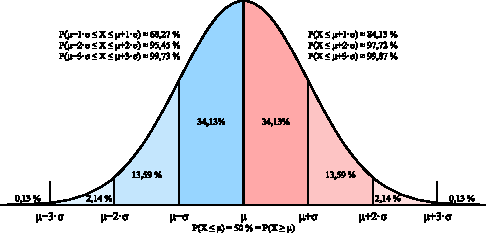
\includegraphics[width=0.9\textwidth]{figures/tschebysheff.pdf}
    \caption{For the normal distribution $P(|X-\mu| \geq 2 \sigma) \approx 1 - 0.9545 \approx 0.05 \leq \frac{1}{2^2}$ - so here
    Tschebysheff's theorem is not very tight.}
    \label{fig:tschebysheff}
\end{figure}

\subsubsection{Proof of Tschebysheff's theorem}
\begin{equation}
    \begin{aligned}
        (k\sigma)^2 \cdot P(|X-\mu| \geq k \sigma) &= \underbrace{\int_{-\infty}^{\mu-k\sigma} (k\sigma)^2 f(x) \, dx}_{\text{note here } (k\sigma)^2 \leq (x-\mu)^2} + \int_{\mu+k\sigma}^{\infty} (k\sigma)^2 f(x) \, dx \\
        &\leq \int_{-\infty}^{\mu-k\sigma} (x-\mu)^2 f(x) \, dx + \underbrace{\int_{\mu-k\sigma}^{\mu + k \sigma} (x-\mu)^2 f(x) \, dx}{\geq 0} + \int_{\mu+k\sigma}^{\infty} (x-\mu)^2 f(x) \, dx \\
        &= \sigma^2
    \end{aligned}
\end{equation}

\subsection{Moment generating functions}
To characterize and compare distributions, we use their moments\footnote{Which under certain conditions can completely and uniquely specify a distribution.}
\begin{equation}
    m_n := E[X^n] = \int x^n f(x) \, dx
\end{equation}
where the mean is the first moment. The \textbf{moment generating function} is
\begin{equation}
    \boxed{M_X(t) := E[\exp(tX)]} = \int \exp(tx) f(x) \, dx
\end{equation}
which is defined if
\begin{equation}
    \exists h > 0: \forall t \in (-h,h): M_X(t) < \infty
\end{equation}
so for instance not for the Cauchy distribution (which does not even have a finite mean).

\bluebox{\textbf{From Taylor expansion to the moments} Consider the series expansion
\begin{equation}
    \exp(tX) = 1 + tX + \frac{t^2 X^2}{2!} + \frac{t^3 X^3}{3!} + \dots + \frac{t^n X^n}{n!} + \dots
\end{equation}
so as of the linearity of the expectation value
\begin{equation}
    E[\exp(tX)] = 1 + tE[X] + \frac{t^2 E[X^2]}{2!} + \frac{t^3 E[X^3]}{3!} + \dots + \frac{t^n E[X^n]}{n!} + \dots
\end{equation}
Now consider $\left.\partial_t M_X(t) \right|_{t=0}$ - it is just $E[X]$.
}

\subsubsection{Calculating moments from the moment generating function}
The $n$-th moment of $X$ is the $n-$th derivative of the moment generating function at $t=0$
\begin{equation}
    m_n := E[X^n] = \left.\frac{d^n M_X(t)}{dt^n}\right|_{t=0}
\end{equation}

\subsubsection{Multidemensional moment generating function}
For the random vector
\begin{equation}
    \vec{X} = \left( \begin{array}{c}
        X_1 \\ X_2 \\ \vdots \\ X_N
    \end{array} \right)
\end{equation}
the moment generating function is
\begin{equation}
    M_{\vec{X}}(\vec{t}) = E[\exp(\vec{t}^T \vec{X})]
\end{equation}

\subsubsection{Example: Moment generating function of the Poisson distribution}
The (discrete) Poisson equation is
\begin{equation}
    P(k;\lambda) = \frac{\lambda^k}{k!} \exp{(-\lambda)}
\end{equation}
so the moment generating function is (using $\exp(x) = \sum_{n=0}^{\infty} \frac{x^n}{n!}$)
\begin{equation}
    \begin{aligned}
        E[\exp(tk)] &= \sum_{k=0}^{\infty} \exp(tk) \frac{\lambda^k}{k!} \exp{(-\lambda)} \\
         &= \exp{(-\lambda)} \sum_{k=0}^{\infty} \frac{\left(\exp(t)\lambda\right)^k}{k!} \\
         &= \exp{(-\lambda)} \exp{\left(\exp(t)\lambda\right)} \\
         &= \exp{\left(\lambda(\exp(t)-1)\right)}
    \end{aligned}
\end{equation}

\subsection{Multivariate probability distributions}
Let us consider the joint probability distribution of multiple RVs
\begin{equation}
    p(x_1, x_2, \dots, x_k) = p(X_1=x_1, X_2=x_2, \dots, X_k=x_k)
\end{equation}
so the probability of a certain combination of outcomes of the RVs.
The normalization is (integrals in the continuous case)
\begin{equation}
    \sum_{x_1} \dots \sum_{x_k} p(x_1, x_2, \dots, x_k) = 1
\end{equation}
The joint cumulative distribution function is
\begin{equation}
    F_{X_1,\dots,X_k}(x_1, x_2, \dots, x_k) = p(X_1 \leq x_1, X_2 \leq x_2, \dots, X_k \leq x_k)
\end{equation}
which is monotonically non-decreasing in all its arguments, bound by $0$ and $1$ and has the limits
\begin{equation}
    \lim _{x_1, \ldots, x_n \rightarrow+\infty} F_{X_1 \ldots X_n}\left(x_1, \ldots, x_n\right)=1 \quad \text { and } \quad \lim _{x_i \rightarrow-\infty} F_{X_1 \ldots X_n}\left(x_1, \ldots, x_n\right)=0 \text {, for all } i \text {. }
\end{equation}

\subsubsection{Multi-categorical distribution}
Consider a setting of multiple possible classes not just failure and success, e.g.
the probability of a randomly chosen farm animal being some species.
\subsubsubsection{Encoding the category by 1-hot encoding}
Consider we have $k$ (exclusive) categories. The naive encoding would be to assign a number to each category,
$y = 1$ for cow, $y = 2$ for donkey, $3$ for sheep, etc. This has two major disadvantages:
\begin{itemize}
    \item it implies an ordering and distance, in this space cow and sheep are farther apart than cow and donkey, which makes no sense
    \item moments of the distribution, e.g. the expected value, are nonsensical
\end{itemize}
We better use \textbf{$1$-hot encoding}, where $k$ categories are encoded in a $k$-dimensional vector with a $1$ at the position of the active 
category and $0$ elsewhere. So for an observation $\vec{y}_i$ (a single data-point), we have
\begin{equation}
    \left[\underline{y}_i\right]_k=\left\{\begin{array}{c}
        1 \text { if } x_i \text { belongs to class } k \\
        0 \text { else }
        \end{array},\right.
\end{equation}
so an observation of class $k$ has the vector
\begin{equation}
    k: \underline{y}_i=\left(\begin{array}{c}0 \\ \vdots \\ 0 \\ 1 \\ 0 \\ \vdots \\ 0\end{array}\right) \leftarrow \text{k-th position}
\end{equation}
where $1$-hot (class exclusivity) means that for any observation
\begin{equation}
    \quad \sum_k\left[\underline{y}_i\right]_k=1
\end{equation}

\subsubsubsection{Categorical distribution}
For $K$ classes with probabilities $\mu_k$, so
\begin{equation}
    \sum_{k=1}^{K} \mu_k = 1, \quad \mu_k \geq 0, \quad \vec{\mu} = \left(\begin{array}{c}
        \mu_1 \\ \mu_2 \\ \vdots \\ \mu_K
    \end{array}\right)
\end{equation}
and the categorical distribution can be written as
\begin{equation}
    p(\vec{y} \mid \vec{\mu}) = \prod_{k=1}^{K} \mu_k^{y_k}, \quad y_k \in \{0,1\} \text{ so that } p(y = k \mid \vec{\mu}) = \mu_k
\end{equation}
So for $K = 2$ we are back at the Bernoulli distribution.

\subsubsubsection{Expectation, variance and covariance of the categorical distribution}
For many observations $\{\vec{y}_i\}_{i=1}^N$ we expect for the categories (entries of $\vec{y}_i$)
\begin{equation}
    \begin{gathered}
    E\left[y_k\right]=\mu_k, \quad \operatorname{Var}\left(y_k\right)=\mu_k\left(1-\mu_k\right) \\
    \operatorname{Cov}\left(y_k, y_l\right)=\underbrace{E\left[y_k y_l\right]}_{=0 \text{ for } k\neq l \text{ as 1-hot}}-E\left[y_k\right] E\left[y_l\right]=-\mu_k \mu_l \text { for } k \neq l \\
    \vec{E}[\vec{y}]=\vec{\mu}, \quad \text { covariance matrix } \vec{\vec{\Sigma}} \in \mathbb{R}^{K \times K}
    \end{gathered}
\end{equation}

\subsubsection{Multinomial distribution}
Consider we cannot only draw from two possibilities (like success and failure) but from $K$ possibilities. For example,
consider $3$ blue, $2$ red and $5$ green balls in an urn and we draw $20$ with replacement. What is the probability
for drawing $10$ green, $5$ blue and $5$ red balls?

The multinomial is given by
\begin{equation}
    \begin{gathered}
        p(x_1,\dots,x_k) = \frac{N!}{x_1! \dots x_k!} \prod_{i=1}^{k} \mu_i^{x_i}, \quad \text{count } x_i \text{ of occurrences of class } i, \quad \sum_{i=1}^{k} x_i = N \\
        \text{in } N \text{ trials}, \quad \text{permutations } x_1! \dots x_k! \text{ within the classes} \\
        \text{parameters } N, \mu_i, \quad \sum \mu_i = 1, \quad \mu_i \geq 0
    \end{gathered}
\end{equation}

\subsubsubsection{Expectation, variance and covariance of the multinomial distribution}
\begin{equation}
    E[x_i] = N \mu_i, \quad \operatorname{Var}[x_i] = N \mu_i (1 - \mu_i), \quad \operatorname{Cov}[x_i, x_j] = -N \mu_i \mu_j \text{ for } i \neq j
\end{equation}

\subsubsection{Multivariate Gaussian distribution}
Consider we have recorded multiple continuous features like temperature, humidity and pressure.
For a feature vector
\begin{equation}
    \vec{x} = \left(\begin{array}{c}
        x_1 \\ x_2 \\ \vdots \\ x_p
    \end{array}\right)
\end{equation}
with mean
\begin{equation}
    \vec{\mu} = E[\vec{x}] = \left(\begin{array}{c}
        E[x_1] \\ \vdots \\ E[x_p]
    \end{array}\right) = \left(\begin{array}{c}
        \mu_1 \\ \vdots \\ \mu_p
    \end{array}\right) \in \mathbb{R}^p
\end{equation}
and covariance matrix\footnote{One can also define the precision matrix $\mat{\Lambda} = \mat{\Sigma}^{-1}$ ($\sim$ more variation $\rightarrow$ less precision).}
\begin{equation}
    \Cov(\vec{X}) = \mat{\Sigma} = \explain{E\left[ (\vec{X} - \vec{\mu}) (\vec{X} - \vec{\mu})^T \right]}{applied elementwise} = E\left[ \vec{X} \vec{X}^T \right] - \vec{\mu} \vec{\mu}^T \in \mathbb{R}^{p \times p}
\end{equation}
so with the elements
\begin{equation}
    \Sigma_{ij} = \Cov(x_i, x_j) = E[(x_i - \mu_i)(x_j - \mu_j)]
\end{equation}
to follow a multivariate Gaussian distribution, $\vec{X} \sim \mathcal{N}(\vec{\mu},\mat{\Sigma})$, means
\begin{equation}
    \phi_{\vec{\mu}, \mat{\Sigma}}(\vec{x})=(2 \pi)^{-\frac{p}{2}}(\operatorname{det} \mat{\Sigma})^{-\frac{1}{2}} \exp \left(-\frac{1}{2}(\vec{x}-\vec{\mu})^T \mat{\Sigma}^{-1}(\vec{x}-\vec{\mu})\right)
\end{equation}
For the case of two features, the Gaussian distribution is illustrated in figure \ref{fig:gaussian2d1} and \ref{fig:gaussian2d2}.

\begin{figure}[!htb]
    \centering
    \includesvg[width=0.9\textwidth]{figures/gaussian2d1.svg}
    \caption{Gaussian distribution in 2D}
    \label{fig:gaussian2d1}
\end{figure}

\begin{figure}[!htb]
    \centering
    \includesvg[width=0.9\textwidth]{figures/gaussian2d2.svg}
    \caption{Gaussian distribution in 2D}
    \label{fig:gaussian2d2}
\end{figure}

\pagebreak